\documentclass[10pt,twocolumn]{article}
\usepackage[letterpaper,margin=0.74in,columnsep=0.25in]{geometry}
\usepackage[T1]{fontenc}
\usepackage{lmodern}
\usepackage{microtype,amsmath,amssymb,booktabs,array,tabularx,graphicx,xcolor}
\usepackage[hyphens]{url}
\usepackage[colorlinks=true,allcolors=blue!45!black]{hyperref}
\usepackage{enumitem}
\setlist{nosep,leftmargin=*}
\setlength{\parskip}{2pt}
\setcounter{dbltopnumber}{2}
\renewcommand{\dbltopfraction}{.90}
\renewcommand{\dblfloatpagefraction}{.75}
\raggedbottom
\hypersetup{pdftitle={Marginal-Cost-Aware Expert Skipping for Fine-Grained MoE Decode},pdfauthor={Research draft}}
\newcommand{\ind}{\mathbf{1}}
\newcolumntype{L}[1]{>{\raggedright\arraybackslash}p{#1}}
\newcolumntype{Y}{>{\raggedright\arraybackslash}X}
\newcommand{\pending}{\textbf{Pending}}
\newcommand{\method}{marginal-cost skipping}
\newcommand{\artifactfigure}[3]{\begin{figure}[t]\centering
\IfFileExists{#1}{\includegraphics[width=\columnwidth]{#1}}{\fbox{\parbox[c][0.48in][c]{0.93\columnwidth}{\centering\small #2}}}
\caption{#3}\end{figure}}
\title{Skip Only What You Would Load:\\Marginal-Cost-Aware Expert Skipping for Fine-Grained MoE Decode}
\author{Research draft}
\date{October 16, 2026}
\begin{document}
\maketitle
\begin{abstract}
In batched mixture-of-experts (MoE) decoding, removing an assignment eliminates an expert's logical weight footprint only if no other token still uses it. We study a budgeted tail-skipping rule that uses this singleton condition. Under independent uniform routing, the singleton-assignment fraction is $(1-k/E)^{B-1}$. Native OLMoE long-decode counters in BF16 and FP8 cover batches 1--64, and BF16 rank-by-gate interventions characterize whole-model loss. On 32 exploratory WikiText-2 validation documents with 32 teacher-forced decode predictions each, the middle-budget policy at $B=8$ reduces logical footprint by 21.65\%, with mean full-vocabulary KL .04595; native top-6 reduces footprint by 17.73\%, with KL .07384. A separate FP8 comparison on the same articles retains this $B=8$ tradeoff: 21.60\% reduction and KL .05506 versus top-6's 17.71\% and .07772, each relative to native FP8. Separate 63-cell CUDA-graph matrices in each format use native-oriented tuning and 2048 fixed outputs per request. At $B=8$, the middle-budget policy lowers measured TPOT/J per token by 11.26/14.87\% in BF16 and 3.87/8.24\% in FP8. At $B=64$, its energy changes by less than .16\% in either format. These are single-run observations on different trajectories from the quality windows. A natural-completion screen on 200 windows from 28 other validation articles reaches the 256-token cap in 94.5--97.5\% of outputs. In a 16-problem GSM8K pilot, the middle- and high-budget policies each answer four correctly versus native's six. Thus the measured execution gains are not established as equal-quality task acceleration. Logical bytes are not DRAM transactions. Independent repeats, full-task and held-out quality evaluation, and the other two target models remain pending.
\end{abstract}

\section{Introduction}
Batched decode shares an expert's weights among tokens assigned to that expert. This sharing creates a mismatch between token-level sparsity and the amount of distinct expert data an execution step needs. A low-contribution assignment can be removed while leaving every expert in the batch active. Conversely, removing the only assignment to an expert can eliminate its entire logical weight footprint from that step. Whether the latter reduces physical memory traffic or time depends on the kernel, caches, quantization, and control overhead.

Our question is narrow: \emph{does conditioning a simple tail-skipping policy on current-batch singleton occupancy improve the measured quality--cost frontier of decode?} We keep the pretrained router, add no learned gate, and do not replace experts with alternatives. The proposed controller counts the returned assignments and spends its gate-mass budget only on tail assignments whose removal makes an expert inactive in that execution batch.

Prior work already provides dynamic expert counts, inference-time skipping, and batch-aware expert reduction. In particular, SERE targets batched decoding through similarity-based re-routing~\cite{sere}. Therefore batch awareness alone is not a contribution claim. Our candidate distinction is the direct use of singleton marginal footprint, combined with an explicit gate-mass budget, without expert-substitution calibration. Its practical value requires measurement.

The current evidence combines an occupancy model, an executable policy, seven-batch OLMoE occupancy measurements and exploratory quality--footprint comparisons at $B=1,8,32$ in BF16 and FP8, and complete single-run graph performance/energy matrices in both formats. The measured tradeoff changes with batching: a singleton-conditioned rule can avoid some quality cost of shared assignments, but it has no reuse-based advantage when $B=1$, and its observed performance effect becomes small at large batches. The quality and performance experiments use different workloads and cannot be joined into an equal-quality performance frontier. The remaining question is whether useful execution gains persist under independent repetition and an explicit application-quality constraint; wider model coverage is also ongoing.

\section{Background and Scope}
Consider one routed MoE layer in one decode execution batch. There are $B$ real tokens, $E$ routed experts, and $k$ distinct expert assignments per token before intervention. Rank $r=1$ denotes the highest routing weight. Shared experts, attention, the router, and other model components remain in the measured full-step cost, but they are not candidates for removal. Padding is excluded from occupancy. If execution partitions a scheduling batch into microbatches, occupancy must describe the actual group sharing an expert kernel; counting across unrelated executions exaggerates reuse.

We distinguish three quantities. \emph{Assignments} count dispatched token--expert pairs. \emph{Logical distinct weight bytes} sum the physical tensor sizes associated with experts that have at least one remaining assignment, counting each expert once. \emph{DRAM bytes} are hardware-observed memory transactions in a defined kernel or step region. The first two can be measured from routing and tensor metadata. Neither is a DRAM counter. Alignment, repeated tiled loads, dequantization, cache hits, and non-weight traffic can cause their changes to differ.

The initial target is single-GPU decode with vLLM 0.26.0. Checkpoint, tokenizer, quantization artifact, and normalization settings are identical within each policy comparison. BF16 and FP8 comparisons on the available RTX PRO 6000 form separate within-format experiments. Other devices and AWQ/NVFP4 are conditional extensions, not completed results.

\section{Singleton Occupancy and Marginal Cost}
\subsection{Inclusion probabilities}
Let $I_{t,e}\in\{0,1\}$ indicate that token $t$ selects expert $e$, and let $N_e=\sum_{t=1}^{B}I_{t,e}$. Define the \emph{token inclusion probability} $q_e=\Pr(I_{t,e}=1)$, so $\sum_e q_e=k$ when exactly $k$ distinct experts are selected. If a normalized slot-frequency statistic $p_e$ is used instead, $p_e=q_e/k$ and $\sum_e p_e=1$. A raw router softmax probability is not generally either of these statistics; top-$k$ selection changes inclusion probabilities.

Under identical independent routing across tokens,
\begin{align}
\Pr(N_e=1)&=Bq_e(1-q_e)^{B-1},\\
u(B)&=\frac{\mathbb{E}[\sum_e\ind\{N_e=1\}]}{Bk}\nonumber\\
&=\frac{1}{k}\sum_e q_e(1-q_e)^{B-1}.\label{eq:singleton}
\end{align}
A singleton expert contributes exactly one singleton assignment. The definition of $u$ therefore refers to the fraction of assignments, not the fraction of active experts. Independence between experts within a token is unnecessary; top-$k$ selection already couples those events. For uniform inclusion $q_e=k/E$,
\begin{equation}
u(B)=(1-k/E)^{B-1}.\label{eq:uniform}
\end{equation}
Likewise, the expected distinct-expert count is
\begin{equation}
\mathbb{E}[D]=\sum_e[1-(1-q_e)^B].
\end{equation}
These are occupancy predictions, not savings forecasts: the gate and rank constraints permit dropping only a subset of singleton assignments.

\subsection{Correlated and heterogeneous tokens}
Real decode batches can share prompts, domains, and generation histories. In the general case,
\begin{equation}
\Pr(N_e=1)=\sum_t\Pr(I_{t,e}=1,\ I_{s,e}=0\ \forall s\ne t).
\end{equation}
Marginal frequencies alone do not determine this joint probability. Even independent but nonidentical tokens require $\sum_t q_{t,e}\prod_{s\ne t}(1-q_{s,e})$. Where per-expert traces are available, measured natural-batch singleton fractions can be compared with both the uniform model and an in-sample fitted $q_e$ model. The long-trajectory counters below lack those marginals and use only the uniform reference. Randomly regrouped trace positions are a correlation diagnostic and are labeled replay; they do not establish natural multi-request decode behavior. Layers and workload classes are retained separately before aggregation.

\subsection{Exact logical footprint change}
Let $w_e$ be the resident bytes of the expert tensors needed by its selected execution format, including attributable scales and metadata. With $D=\sum_e\ind\{N_e>0\}$,
\begin{equation}
W=\sum_e w_e\ind\{N_e>0\}.
\end{equation}
For a single removed assignment $(t,e)$, holding the others fixed,
\begin{equation}
c_{t,e}=w_e\ind\{N_e=1\}.
\end{equation}
For an arbitrary simultaneous removal set $S$, the exact footprint decrease is
\begin{equation}
\Delta W(S)=\sum_e w_e\ind\{N_e>0\}\ind\{N_e-|S_e|=0\},\label{eq:setcost}
\end{equation}
where $S_e$ contains removed assignments to $e$. Initial marginal costs are additive for our singleton-only policy, but not for arbitrary global-$k$ or threshold policies: several removed assignments can jointly empty a previously shared expert. All policies are therefore evaluated with before/after counts using Eq.~\eqref{eq:setcost}, avoiding a bias against the baselines.

For bandwidth-dominated expert execution, $W/\beta$ is a useful explanatory scale with effective bandwidth $\beta$. It is not a measured duration, a universal lower bound, or an end-to-end speedup estimate. Smaller $W$ may coexist with worse latency if control, launches, or tile efficiency dominate.

\section{Characterization}
\subsection{The batch opportunity region (F1)}
Table~\ref{tab:model} gives exact values from Eq.~\eqref{eq:uniform}. Increasing $E/k$ extends the range where singleton assignments are common under the stated assumptions. The $E/k=32$ row is an analytical geometry, not a measurement of a third model. Models with the same ratio can differ due to skew, rank-specific routing, correlation, shared experts, and kernel granularity.
\begin{table}[t]
\centering\small
\caption{Analytical singleton assignment fraction under independent uniform routing. These values are not measurements.}\label{tab:model}
\begin{tabular}{r r r r r r}\toprule
$E/k$ & $B=1$ & $8$ & $16$ & $32$ & $64$\\\midrule
8 & 1.000 & .393 & .135 & .016 & .0002\\
16 & 1.000 & .637 & .380 & .135 & .017\\
32 & 1.000 & .801 & .621 & .374 & .135\\\bottomrule
\end{tabular}
\end{table}

\begin{figure*}[tp]\centering
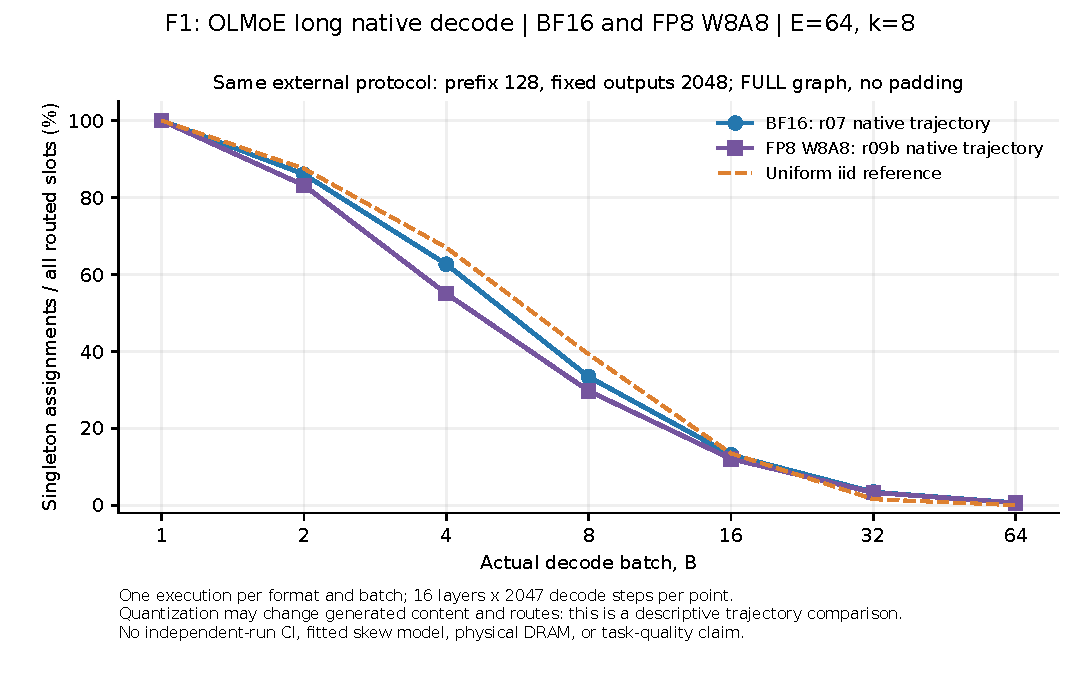
\includegraphics[width=.78\textwidth,trim=0 45bp 0 25bp,clip]{../figures/f1_long_decode_fp8_r09b/F1_format_comparison.pdf}
\caption{F1: native OLMoE long-decode occupancy in BF16 (r07) and FP8 W8A8 (r09b). Each $B=1,2,4,8,16,32,64$ uses 128 prefix tokens and 2048 fixed outputs: 2047 decode steps across 16 routed layers, or 32,752 layer events and $262{,}016B$ slots. Counted replays match their performance transcripts. Each format supplies one execution per batch, without independent-run uncertainty. The dashed curve is the uniform iid reference.}\label{fig:occupancy}
\end{figure*}
Figure~\ref{fig:occupancy} measures both formats' native-generated performance trajectories under the same external protocol, with EOS ignored and no decode padding. The first output follows prefill and is excluded. For increasing $B$, BF16 singleton fractions are 100\%, 86.04\%, 62.64\%, 33.41\%, 13.12\%, 3.45\%, and .649\%; FP8 fractions are 100\%, 83.15\%, 55.01\%, 29.74\%, 12.06\%, 3.32\%, and .605\%. At $B=8$, both are below the uniform prediction of 39.27\%; at $B=32,64$, both exceed 1.59\% and .0222\%. The uniform curve is an explanatory reference, not a calibrated occupancy forecast.

The source cohorts overlap across batch sizes; at $B=64$, 64 distinct WikiText windows come from 60 articles. Tokens and layers are not independent system repetitions. These counters retain per-layer singleton totals but lack complete per-expert inclusion marginals. We therefore fit no skew curve and cannot separate skew from within-batch correlation. FP8 can change generated content and later routes; the matched external protocol does not isolate a direct quantization effect. Singleton opportunity alone is not measured DRAM savings or a quality guarantee. DeepSeek-V2-Lite has 64 routed experts and $k=6$, distinct from the illustrative $E/k=32$ geometry.

Earlier short captures used 32-token prefixes/eight decode steps in BF16 and 128-token prefixes/16 steps in FP8. Those artifacts describe early decode states; the present full trajectories cover later policy-generated states. Differences in prefixes and trajectories prevent attributing short-versus-long differences to observation length alone.

\subsection{Tail dropping and quality (T1)}
Quantizing a tail expert and dropping it are different perturbations. Historical rank-tail quantization evidence motivates examining tail ranks, but does not establish a safe skipping budget. The recovered historical drop row mixes BF16 head experts, FP8 middle experts, and dropped tail experts. Its legacy KL reduction sums token errors within each sequence. This mixed-format intervention and metric convention are not a substitute for a pure-drop T1 on the current checkpoint. T1 measures complete next-token distributions and ground-truth loss after dropping specified ranks, with the model's normalization convention held fixed. Gate bins are defined on pre-intervention selected weight mass; the table retains layer, rank range, sample count, dropped mass, and policy configuration. Initially we use full-vocabulary $D_{\rm KL}(P_{\rm base}\Vert P_{\rm policy})$ and PPL on common teacher-forced contexts. Conditional layer-output error is diagnostic and is not labeled full-model token KL.

Each T1 cell is a separately executed intervention. The initial diagnostic removes only assignments in one rank and one half-open gate interval: $r\in\{5,6,7,8\}$ in the paper's one-based convention, and $g\in[0,.025)$, $[.025,.05)$, $[.05,.1)$, or $[.1,.2)$. The executable configuration uses zero-based ranks $4$--$7$, sets a unit mass budget, and does not impose the singleton constraint. All other ranks and gate intervals are retained. We record skipped-slot and dropped-mass counts; an empty cell is reported as having no selected events, not as showing that removal is safe. The first small validation sample is exploratory.

This experiment estimates the whole-model consequence of repeatedly applying one bin-specific rule across routed decode layers and positions. It is not an isolated single-layer or single-event causal cost, because earlier interventions can change later hidden states and gates. We do not assign the KL of a multi-rank intervention to its individual ranks after the run, sum cell effects, or divide total KL by event count to claim additive per-event loss. The executable arms and resolved parameters are saved with every run.

\paragraph{Measured validation interventions.}
Table~\ref{tab:drop} reports the 16 separately executed rules on the current OLMoE BF16 checkpoint at $B=8$. Every rule uses the same 32 validation articles, a 128-token prefix, and 32 genuine decode predictions per article: 1,024 output-token observations and 16,384 token-layer opportunities. The native control has pooled-window PPL 9.79070. Raw token targets and baseline NLL are paired by document and position; worker counters agree with the recorded summaries. All cells have selected events, although some are rare.

For gates below .025, ranks 5--8 incur only 9, 21, 48, and 118 skips, with mean KL $2.46\!\times\!10^{-5}$ to $3.61\!\times\!10^{-4}$. These small aggregate losses coincide with few interventions and do not establish a generally safe rank. In the $[.05,.1)$ bin, the four ranks incur 6,781--14,529 skips and mean KL .02677--.05318. Rank 5 in $[.1,.2)$ has 9,451 skips, 6.55\% mean removed mass per token-layer, KL .10149, and PPL increase .50749. Rank 8 in that same gate interval has only 193 skips and KL .00248. Comparing these totals without their action counts would confound action frequency with conditional sensitivity. Negative observed NLL or PPL changes in some cells are validation outcomes, not evidence of quality improvement on held-out tasks.

\begin{table*}[t]\centering\footnotesize
\caption{T1: separate rank/gate interventions in OLMoE BF16 at $B=8$. Each row uses the same 32 validation documents, 1,024 decode predictions and 16,384 token-layer opportunities in one run. KL is full-vocabulary KL(native$\Vert$policy); PPL uses pooled NLL. $\bar m$ is mean removed selected mass per token-layer. These whole-model effects are not additive event costs.}\label{tab:drop}
\begin{tabular}{r l r r r r r}\toprule
Rank & Gate interval & KL & $\Delta$NLL & $\Delta$PPL & Skipped slots & $\bar m$ (\%)\\\midrule
5 & [0, 0.025) & 2.4555e-05 & 0.000128 & 0.0012533 & 9 & 0.001012 \\
5 & [0.025, 0.05) & 0.00079752 & 0.0028337 & 0.027783 & 71 & 0.01832 \\
5 & [0.05, 0.1) & 0.034685 & 0.024352 & 0.24135 & 6,781 & 3.594 \\
5 & [0.1, 0.2) & 0.10149 & 0.050536 & 0.50749 & 9,451 & 6.551 \\
6 & [0, 0.025) & 6.7955e-05 & -0.00023016 & -0.0022531 & 21 & 0.002357 \\
6 & [0.025, 0.05) & 0.0015809 & 0.00069925 & 0.0068485 & 273 & 0.07137 \\
6 & [0.05, 0.1) & 0.053181 & 0.010888 & 0.10719 & 12,056 & 6.09 \\
6 & [0.1, 0.2) & 0.038353 & 0.010323 & 0.1016 & 4,044 & 2.669 \\
7 & [0, 0.025) & 0.00018611 & -0.00020704 & -0.0020268 & 48 & 0.005361 \\
7 & [0.025, 0.05) & 0.0032335 & -0.0027579 & -0.026965 & 785 & 0.2026 \\
7 & [0.05, 0.1) & 0.044293 & 0.029786 & 0.29601 & 14,529 & 6.858 \\
7 & [0.1, 0.2) & 0.01017 & -0.0084947 & -0.082817 & 1,057 & 0.6786 \\
8 & [0, 0.025) & 0.00036069 & 0.00087005 & 0.0085221 & 118 & 0.01302 \\
8 & [0.025, 0.05) & 0.0052182 & 0.0064445 & 0.0633 & 1,744 & 0.4476 \\
8 & [0.05, 0.1) & 0.026772 & 0.017372 & 0.17157 & 14,343 & 6.305 \\
8 & [0.1, 0.2) & 0.0024825 & -0.0011002 & -0.010766 & 193 & 0.1223 \\
\bottomrule\end{tabular}\end{table*}

Teacher-forced quality must use the intended decode grouping when the policy depends on batch composition. Applying the controller to an entire prefill sequence produces different singleton counts and answers a different question. Free generation additionally records natural EOS, capped sequences, failures, and output lengths. These checks complement, rather than replace, task evaluation.

\section{Design and Implementation}
\subsection{Decision rule}
For each token, let $a_{t,r}$ be the selected pre-intervention routing weight and define $g_{t,r}=a_{t,r}/\sum_j a_{t,j}$ for the budgeting decision. A candidate assignment must satisfy
\begin{equation}
r\ge r_0,\quad g_{t,r}\le\tau,\quad N_{e(t,r)}=1.
\end{equation}
Candidates are considered in a deterministic tail-first order, accepting one only if cumulative dropped mass remains at most $m$. At least one assignment is retained. Tie-breaking must be fixed. The constraint $\sum_{r\in S_t}g_{t,r}\le m$ is a gate-mass bound; it is not a bound on token KL, perplexity, or task loss. We do not assume that errors add independently across layers or steps.

For models that renormalize selected routing weights, the surviving weights are renormalized after dropping. Otherwise their original surviving values and any model-specific scaling are preserved. The normalization used to define the decision budget does not by itself authorize changing the model's output normalization. A disabled controller returns the native route and weights.

The inspected OLMoE installation has 16 \texttt{FusedTopKRouter} layers with \texttt{renormalize=False}; its BF16 routed tensors occupy 12,582,912 bytes per expert. Accordingly, its main quality experiments leave surviving routing weights unchanged after dropping. They are not described as ``drop and renormalize.'' The normalized fractions used for $g$ and $m$ remain decision quantities. Any additional survivor-renormalization diagnostic would be a separately labeled intervention and is not part of the main comparison.

\subsection{Execution integration}
The vLLM 0.26 router abstraction returns expert identifiers and weights through \texttt{FusedMoERouter.select\_experts}; the runner owns the router and routed-expert implementation. The controller attaches after native expert selection. The installed source and actual backend are recorded for each run; the historical \texttt{layer.py} entry point is not assumed to cover every backend.

The logical removed slot uses identifier $-1$ and weight zero. This representation alone does not demonstrate that the native dispatch path accepts negative IDs. An expert-map result of $-1$ at the block level is not a contract allowing $-1$ as input to a histogram. Our path filters removed slots before native alignment and leaves their output contributions zero. Backend tests compare against explicit reference evaluation, verify all-kept/removed-tail cases and mixed occupancy, and inspect launched work. No unsupported path is labeled accelerated.

The implemented alignment maps removed identifiers to one extra sentinel expert before the native histogram, then maps its blocks to $-1$. Both native Triton GEMMs explicitly zero those output blocks and return before expert-weight loads. All 15 synthetic BF16 checks across $B=1,2,8,32,64$ and three policies passed: relative output L2 against an independent FP32 expert reference was .00364--.00418. Replacing every unused expert's weights with NaNs left outputs finite and exactly unchanged. These checks establish the tested execution behavior; they do not measure hardware DRAM traffic. The package has also been built and imported from an isolated installation.

\paragraph{Graph replay and FP8 execution.}
For BF16, the fixed-policy CUDA-graph worker passes eager-versus-graph output and counter parity at real batches $B=3,5$ captured into buckets 4 and 8. Every checked decode step executes in FULL graph mode; the dense graph also matches the native graph outputs. A GPU actual-token scalar excludes padding from policy decisions and logical counters. Padding routes otherwise pass through unchanged, so a real-token logical singleton is not necessarily a physical singleton in a padded kernel. The main powers-of-two performance matrix therefore requires verified unpadded execution. These checks establish graph execution behavior, not graph speedup.

Online FP8 W8A8 conversion of the same checkpoint now has completed eager quality comparisons at $B=1,8,32$, each on 32 articles and 1,024 scored decode predictions per arm. Native-versus-dense identity is exact in the recorded KL and NLL metrics. The installed routed-expert tensors use 6,291,456 weight bytes plus eight scale bytes per expert, compared with 12,582,912 BF16 bytes. Global-tail and marginal actions execute through the inspected Triton path. A subsequent native control, with no skip policy and route counting disabled, still produces different eager and graph outputs at $B=3,5$ padded into buckets 4 and 8; the strict parity check remains failed. The observation therefore does not require skipping, but it neither identifies quantization scales as its cause nor establishes a padding fix. At the seven exact capture buckets $B=1,2,4,8,16,32,64$, dense and marginal arms each pass eager/graph output and counter parity, and native/dense outputs agree within each execution mode. The completed FP8 performance matrix below uses only these seven unpadded buckets. These execution checks do not establish cross-format quality equivalence.

Counters record pre/post assignment counts, distinct experts, singleton candidates, removed mass, and $W$ for each real decode batch. The same counter logic applies to every policy. Route-statistics collection is disabled in the timed graph pass and collected in a separate replay. The occupancy computation needed by the decision, budget selection, alignment, and normalization remain part of policy cost; their times are not subtracted from full-step latency.

\subsection{Concrete behavior}
Suppose two tokens select $\{A,B\}$ and $\{A,C\}$, with $A$ highest-ranked for both. Removing tail $B$ removes $w_B$ of logical footprint. If both instead select $\{A,B\}$, removing $B$ for only one token leaves the footprint unchanged. A global policy removing both $B$ assignments can save $w_B$ jointly; singleton-only skipping deliberately does not exploit that action. This restriction simplifies the decision and constrains quality interventions, but can leave useful opportunities to a strong baseline. Its net value is empirical.

\section{Evaluation}
\subsection{Comparisons and measurement}
The initial matrix uses $B\in\{1,2,4,8,16,32,64\}$ and native top-$k$, global top-$(k-j)$ for valid $j\in\{1,2,4\}$, batch-independent gate thresholding, and \method. Within each format, the completed performance matrix shares one native-oriented kernel configuration across all arms; FP8 uses its own tuning, not the BF16 file. A pending ablation will remove only the singleton condition while keeping rank, gate, mass budget, and normalization identical, to isolate the value of occupancy information. Full AdapMoE is not equated with the pure gate-threshold baseline: sensitivity gating, prefetching, and cache allocation are separate components. Adapted nearest-neighbor components are explicitly labeled as such.

Requested model coverage is OLMoE, Qwen3-30B-A3B, and DeepSeek-V2-Lite. Actual routed/shared expert counts and tensor sizes come from the loaded configurations. Each model/format comparison uses the same weight artifact for quality and performance. Measurements currently use one RTX PRO 6000 Blackwell Server Edition and vLLM 0.26.0. OLMoE BF16 and online FP8 W8A8 have complete three-batch eager quality comparisons and seven-batch graph performance matrices below. Qwen3-30B-A3B, DeepSeek-V2-Lite, and broader task-quality comparisons remain pending.

TPOT is measured across defined decode windows, separately from prefill, compilation, and warm-up. Full generation measurements retain all scheduled requests and record termination causes. Fixed-token replay is reported as controlled work and does not establish application utility. Runs, not tokens sharing a run, are the repetition units. Report individual repeated-run values or uncertainty, and use local A/A variation to interpret the effect. Interleave policy order to reduce time drift. The controller can change later routes and output lengths, so complete policies execute their own trajectories.

Joules per token uses time-aligned NVML power samples integrated over the measurement window, with generated-token counts from that window. Where available, the device cumulative-energy counter is an additional check. Report sampling cadence, warm-up, duration, and whether energy is gross device energy. Short windows can be distorted by power averaging; aggregate sufficiently long steady decode regions. Neither wattage nor latency alone is converted into measured energy.

\begin{table*}[t]\centering\footnotesize
\caption{T2: action-level comparison based on primary papers and author releases checked on October 16, 2026. ``No'' means the described decision does not explicitly use current decode-batch singleton marginal footprint. It does not mean the system cannot benefit from reuse.}\label{tab:related}
\begin{tabularx}{\textwidth}{L{0.12\textwidth} L{0.24\textwidth} L{0.24\textwidth} L{0.14\textwidth} Y}\toprule
Method & Decision signal & Action & Training / calibration & Singleton marginal bytes\\\midrule
AdapMoE~\cite{adapmoe} & Token gate weight and layer Fisher sensitivity & Top-2 to top-1 gating; separate cache/prefetch management & Sensitivity calibration & No; offload loading objective\\
NAEE~\cite{naee} & $g_2/g_1$ versus layer-calibrated ratio & Drop second expert; renormalize & Ratio calibration; no gate retraining & No\\
Ada-K~\cite{adak} & Token representation through learned allocator & Choose token-specific $k$ & PPO allocator training & No\\
MoE++~\cite{moepp} & Learned router with preceding-layer gating residual & Select FFN, zero, copy, or constant experts & Architecture training & No\\
DynMoE~\cite{dynmoe} & Token--expert similarity and learned thresholds & Top-any routing; add/remove experts during training & Gate/model training & No\\
Expert Choice~\cite{expertchoice} & Expert affinity ranking across token group & Each expert takes a capacity-limited token set & Routing/model training & Batch-coupled; no singleton cost rule\\
SERE~\cite{sere} & Batch primary union and calibrated expert similarity & Re-route secondary assignments to primary experts; retain critical ones & Similarity calibration; no retraining & Batch-aware union reduction, different action\\
This design & Tail rank, gate mass, current $N_e=1$ & Drop singleton assignment within per-token mass budget & Threshold calibration only & Yes for logical footprint; DRAM effect unmeasured\\\bottomrule
\end{tabularx}\end{table*}

\subsection{Exploratory quality--footprint frontier (F3)}
We use 32 distinct WikiText-2 validation articles for all three batch sizes, with 128 prefix tokens and 32 scored decode predictions per article. A logits processor records full-vocabulary $D_{\rm KL}(P_{\rm native}\Vert P_{\rm policy})$ and target NLL before forcing the next corpus token. The first prediction follows prefill and is excluded; the next 32 predictions exercise real decode. Identical emitted transcripts are imposed by this protocol and are not a free-generation equivalence result. PPL is $\exp(\sum\mathrm{NLL}/1024)$ over the selected windows, not whole-corpus WikiText perplexity.

The comparison contains native top-8, native top-$(8-j)$ for $j=1,2,4$, two gate-only policies, and three marginal policies. A separate dense identity arm supplies native-footprint counters and matches native NLL/KL. The gate-only settings are $(\tau,m)=(.05,.10)$ and $(.15,.30)$. Marginal low/mid/high use ranks 5--8 and $(\tau,m)=(.05,.10),(.10,.20),(.15,.30)$. Gate-only routing has no rank or singleton condition; it is a simple threshold baseline, not a controlled singleton-only ablation or a full AdapMoE reproduction. All policies preserve OLMoE's unnormalized surviving weights.

\begin{figure*}[tp]\centering
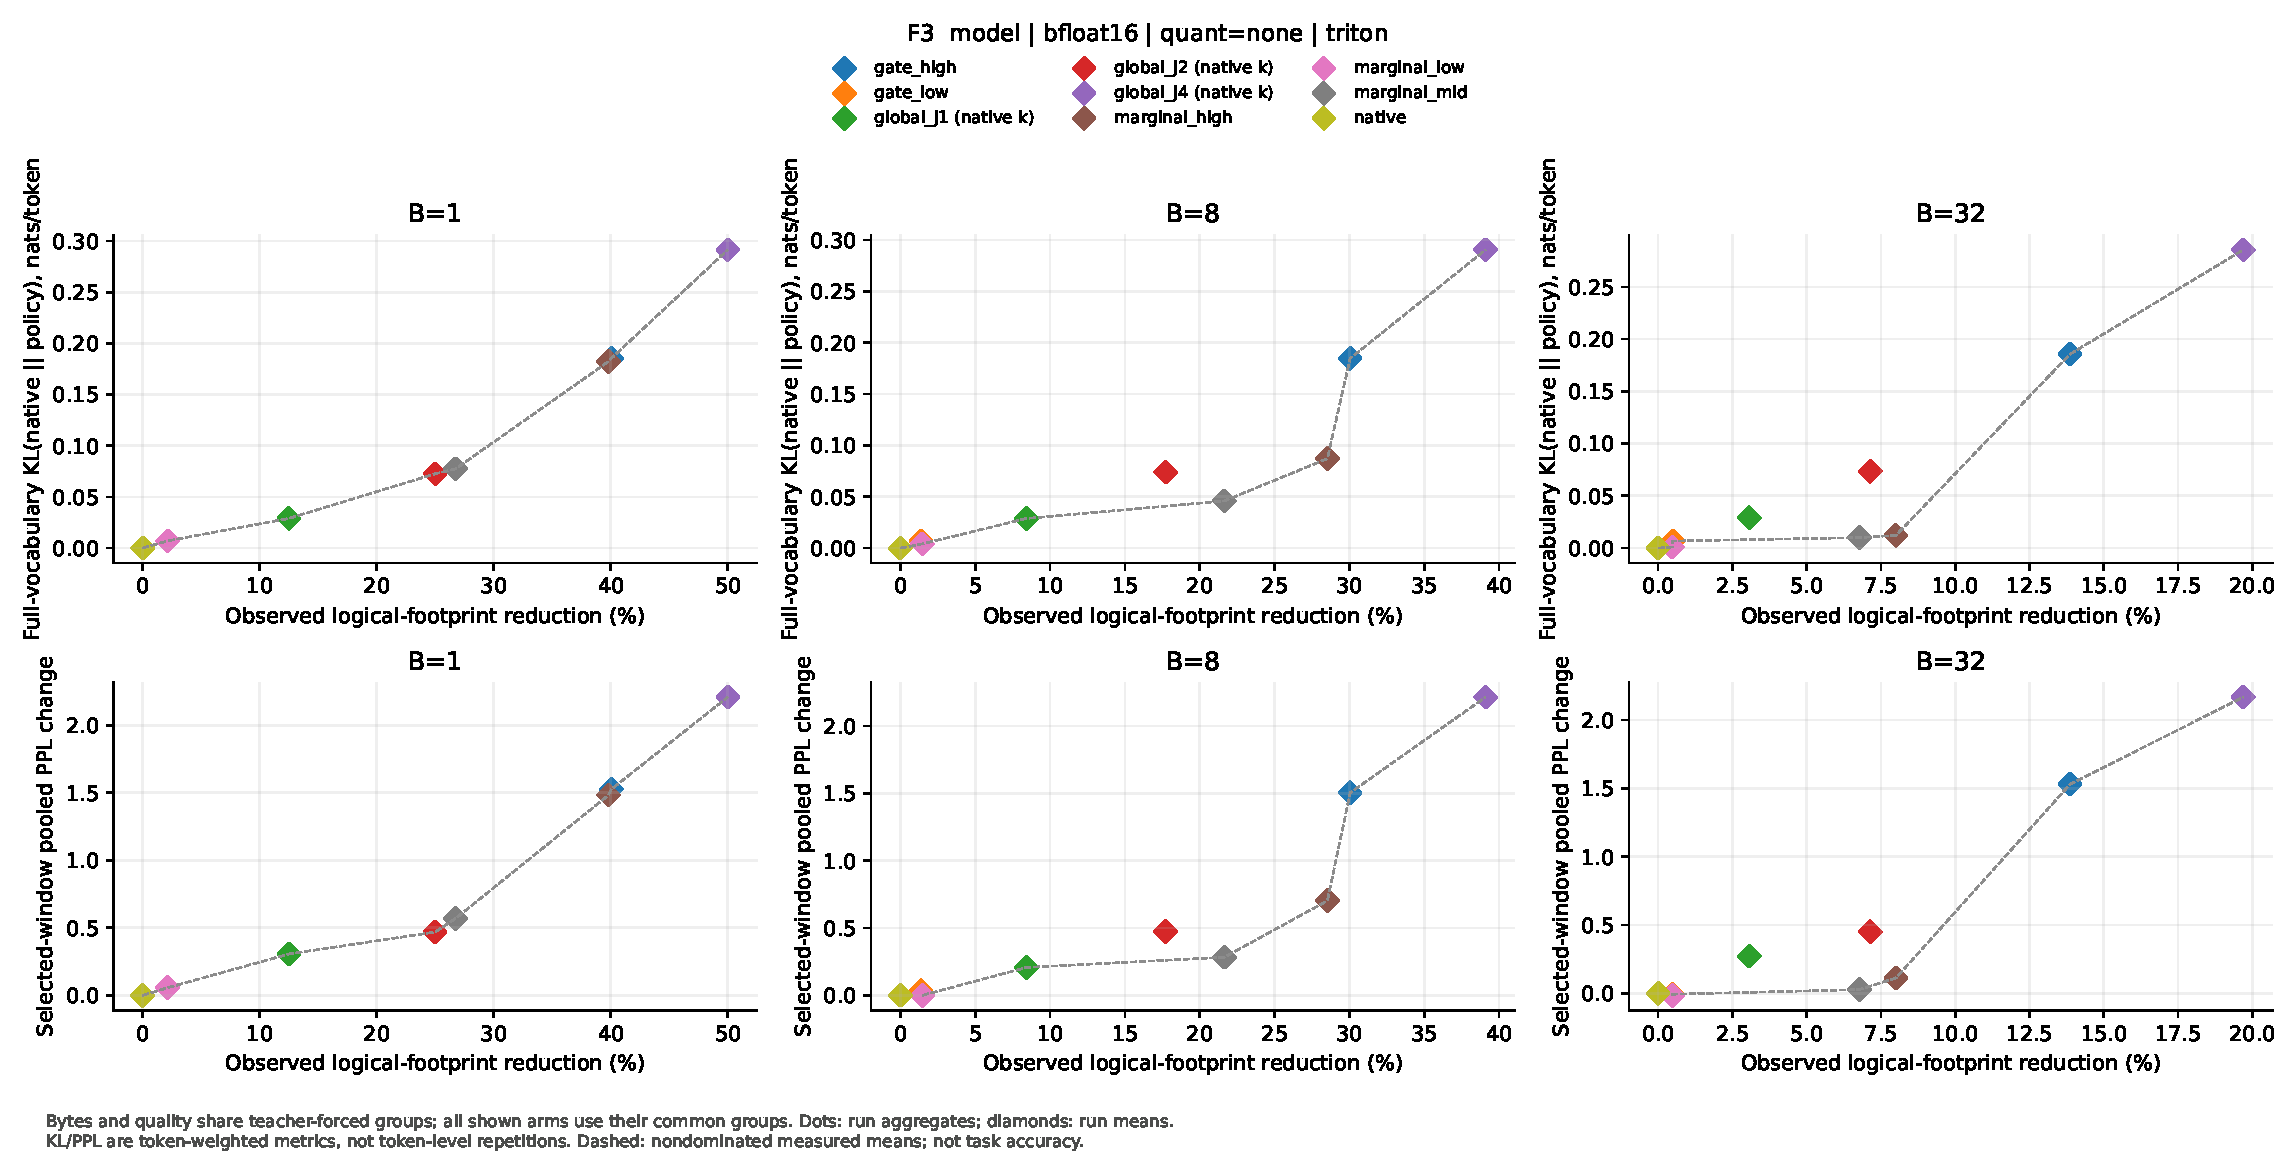
\includegraphics[width=\textwidth]{../figures/quality_r06/F3_model_bfloat16_quant_none_triton_0e13ece6.pdf}
\caption{F3: OLMoE BF16 validation exploration on the same 32 articles, with 32 genuine decode predictions each. Each batch size has one source execution; its points aggregate 32, four, or one cohort at $B=1,8,32$, respectively. Logical bytes and quality come from each policy's teacher-forced trajectory, with native dense counters as the common denominator. Lower right is preferable. Dashed frontiers are descriptive measured means, without task-accuracy or statistical-superiority claims.}\label{fig:quality-r06}
\end{figure*}

Figure~\ref{fig:quality-r06} uses $x=1-W_{\rm policy}/W_{\rm native}$, where each $W$ is the sum of counted distinct expert weight bytes across corresponding layers and steps. Both policies' later routes may differ even with fixed input tokens; a candidate's own pre-intervention footprint is not substituted for the native denominator. Hardware DRAM traffic has not been measured. All three comparisons retain 1,024 paired predictions per arm; raw artifact checks validate document/position pairing and counted populations. Documents are the independent corpus sampling units, while the four $B=8$ cohorts share one system execution and are not independent run repetitions.

At $B=8$, marginal-mid reduces logical bytes by 21.65\%, with KL .04595 and $\Delta$PPL .28242. Native top-6 ($j=2$) reduces bytes by 17.73\%, with KL .07384 and $\Delta$PPL .47457. This measured point favors the count-conditioned rule on both axes, although 22 of 32 documents have higher NLL than native; the aggregate comparison is not pointwise quality preservation. At $B=32$, marginal-high reduces bytes by 8.00\%, with KL .01213 and $\Delta$PPL .11264, versus top-6's 7.14\%, .07348, and .45157. Marginal-mid at $B=32$ uses a smaller intervention: 6.77\% byte reduction, KL .01001, and $\Delta$PPL .02823. These quality observations do not certify the different, longer performance workload below.

The $B=1$ comparison supplies a boundary: marginal-mid reduces bytes by 26.73\% versus top-6's 25\%, but has larger KL (.07740 versus .07259) and $\Delta$PPL (.56846 versus .46888). When all assignments are singletons, occupancy does not screen out shared work. The sparse marginal-low policy at $B=8$ has $\Delta$PPL $-.00090$, which is too small and too exploratory to label a quality gain. Native window PPL itself is 9.80727, 9.79070, and 9.82602 across the three batch sizes because numerical execution can differ; every reported delta uses the native run at its own $B$.

\begin{figure*}[tp]\centering
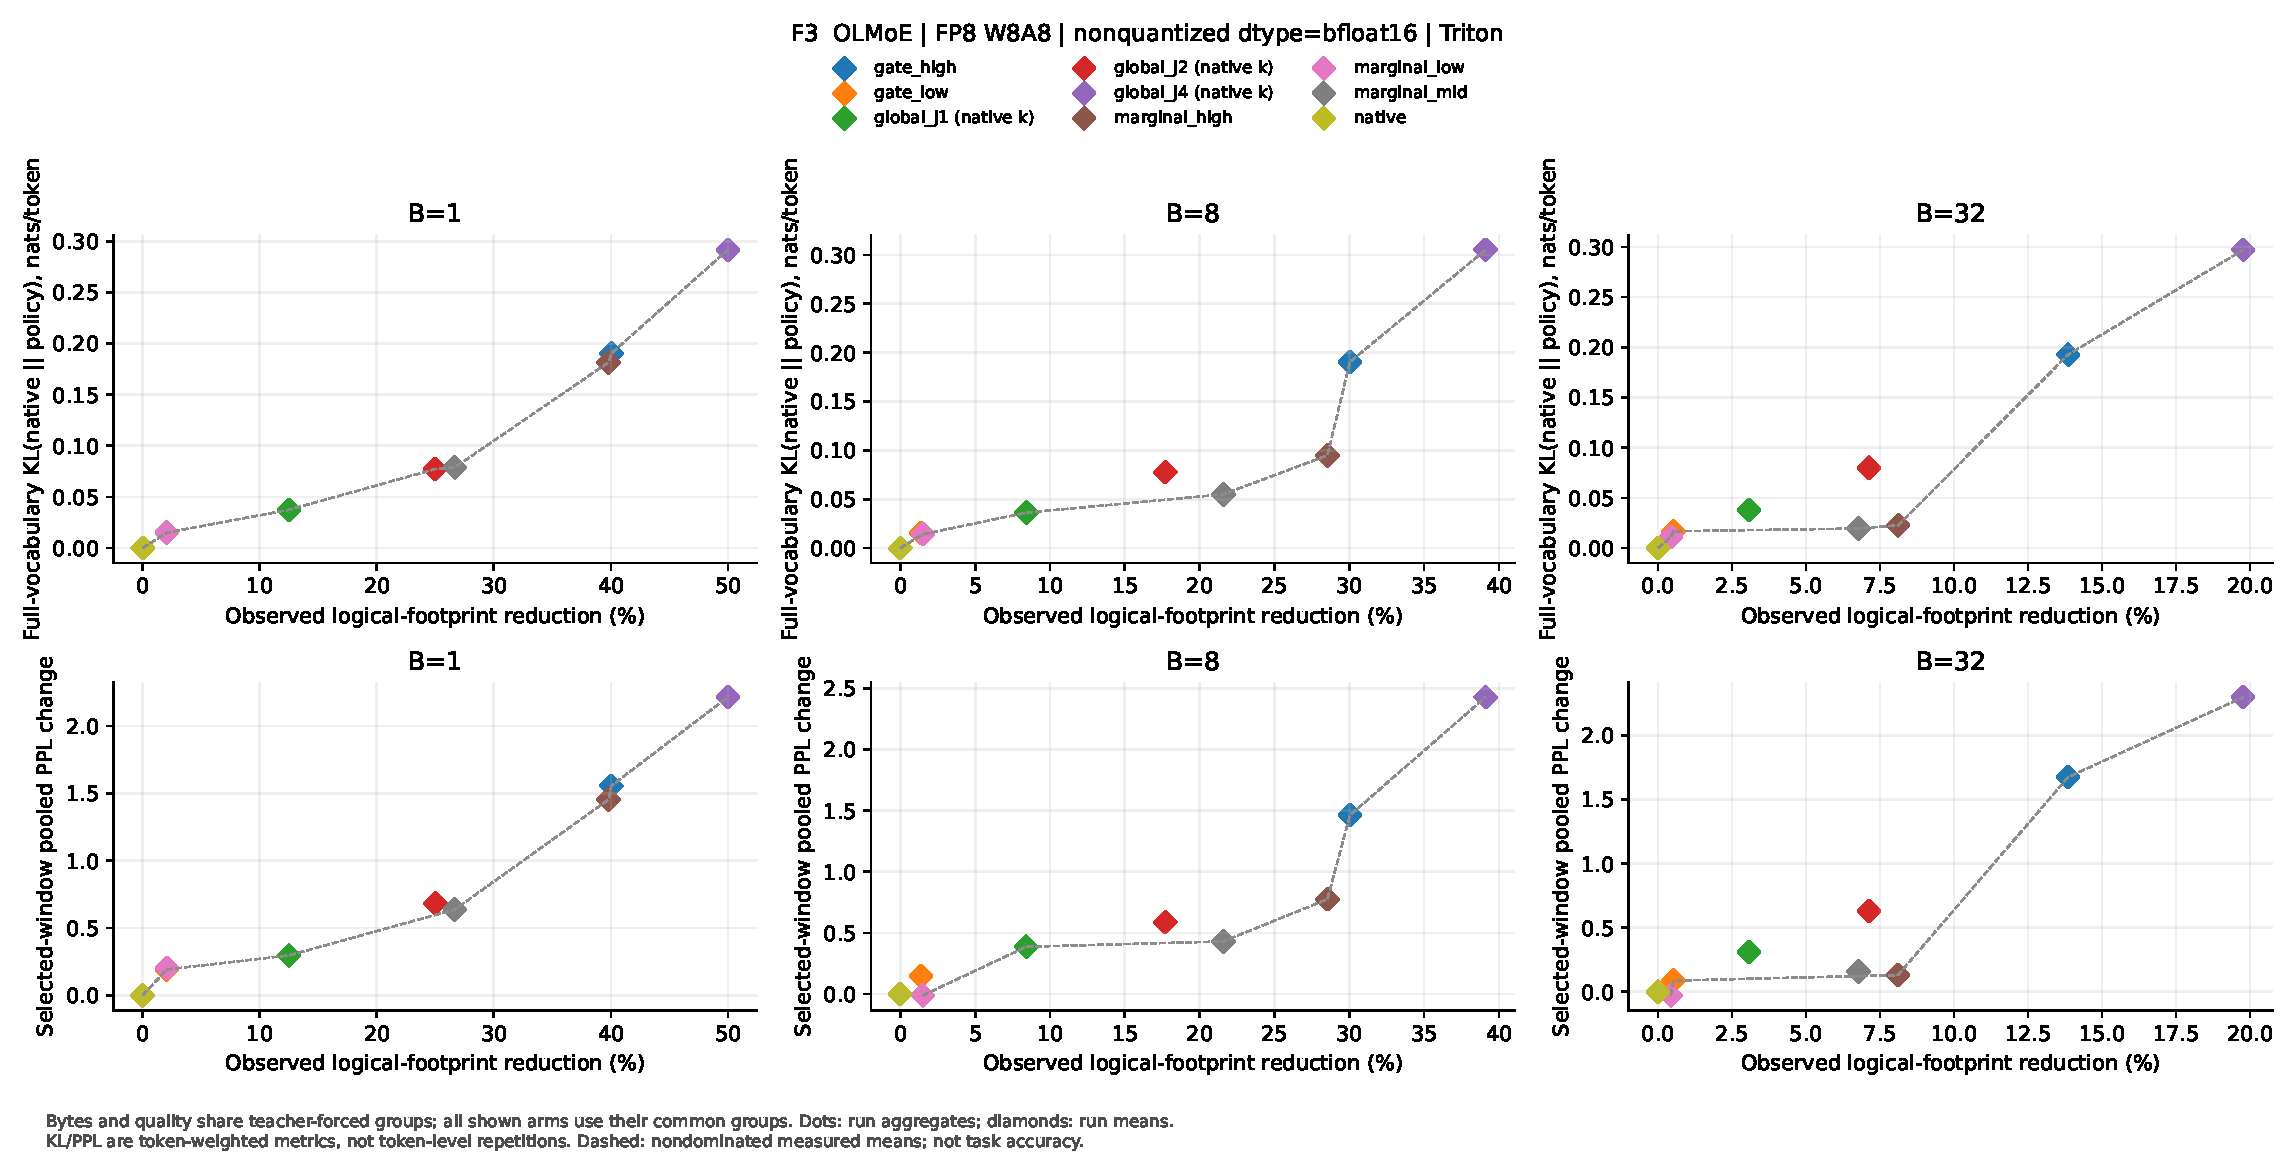
\includegraphics[width=\textwidth]{../figures/quality_fp8_r09/F3_OLMoE_FP8_W8A8_nonquantized_dtype_bfloat16_Triton_9cedcac3.pdf}
\caption{F3 in OLMoE FP8 W8A8: the same 32 validation articles and teacher-forced window protocol as BF16, evaluated against native FP8 separately at each batch size. The nonquantized model dtype remains BF16; routed weights/activations use FP8. Each point aggregates 1,024 scored decode predictions from one source execution. The independent sampling unit is the article, not a token or cohort. Lower right is preferable; the frontiers describe observed means, not task accuracy or an independent confirmation.}\label{fig:quality-fp8-r09}
\end{figure*}

\paragraph{Within-format FP8 comparison.}
Figure~\ref{fig:quality-fp8-r09} uses the same 32 articles, prefix lengths, scored positions, and policy settings in online FP8 W8A8. Each batch size again retains 1,024 predictions per arm in 32, four, or one cohort. For all three batch sizes, the dense identity arm has recorded mean/minimum/maximum KL and $\Delta$NLL exactly zero, with NLL and PPL identical to native. Native FP8 PPL is 9.59947, 9.63869, and 9.70590 at $B=1,8,32$. Every delta and logical-footprint ratio uses native FP8 at its own batch size; these are not cross-format KL measurements or evidence that FP8 improves task quality.



At $B=8$, marginal-mid saves 21.60\% of logical bytes with KL .05506 and $\Delta$PPL .43122, versus top-6's 17.71\%, .07772, and .58810. Thus the observed two-axis advantage persists, with different quality costs. At $B=32$, marginal-high gives 8.11\%, .02265, and .13000 versus top-6's 7.13\%, .07999, and .62938; marginal-mid gives 6.77\%, .01960, and .15689. At $B=1$, marginal-mid saves 26.67\% versus 25\%, but its KL is slightly larger (.07884 versus .07725), while $\Delta$PPL is smaller (.63747 versus .68383). There is no uniform quality-metric advantage at that batch size. Low-budget perturbations also change: marginal-low at $B=32$ has KL .01089 in FP8 versus .00096 in BF16, each relative to its own native distribution. The BF16 thresholds therefore do not supply a cross-format quality guarantee. These exploratory windows do not establish FP8 task gains or quality-matched performance.

The validation articles support exploration only. Separate WikiText test articles remain held out for confirmation. The natural-completion experiment below uses a disjoint set of validation articles; its repeated-text screen is separate from task accuracy.

\subsection{Natural completion and task-quality screening}
The completed BF16 natural-generation family in r08b evaluates all ten arms on the same 200 distinct 128-token prefixes. They are selected from nonoverlapping 256-word windows of 28 WikiText validation articles, excluding the 32 articles used by T1/F3 and all WikiText test articles. Thus 200 windows are not 200 independent articles, and neither windows nor their tokens are independent system repetitions. Generation uses raw text completion without a chat template, greedy sampling, EOS enabled, no minimum output length or repetition penalty, and a 256-token maximum. Cohorts admit at most eight requests and drain naturally; the actual decode batch can shrink as requests finish. This eager evaluation is not the fixed-length graph benchmark in F2/F4.

\begin{table*}[tp]\centering\small
\caption{Natural-completion screen: 200 prompts from 28 validation articles per arm, one execution family. EOS and cap counts sum to 200; every arm has zero failures and zero other-stop cases. Mean output length includes capped completions. $R_4$ is the mean repeated token-4gram ratio over the $n_4$ eligible outputs. Flag counts use all 200 outputs and are descriptive, not correctness judgments.}\label{tab:free200}
\begin{tabular}{lrrrrrr}\toprule
Policy & EOS & 256-token cap & Mean tokens & Mean $R_4$ & $n_4$ & Flags\\\midrule
Native top-8 & 8 & 192 & 251.63 & .26306 & 200 & 39\\
Dense identity & 8 & 192 & 251.63 & .26306 & 200 & 39\\
Native top-7 & 6 & 194 & 253.40 & .29040 & 200 & 48\\
Native top-6 & 7 & 193 & 253.15 & .25483 & 200 & 30\\
Native top-4 & 9 & 191 & 249.68 & .27242 & 200 & 37\\
Gate-low & 11 & 189 & 251.24 & .26777 & 200 & 40\\
Gate-high & 11 & 189 & 248.50 & .26735 & 199 & 38\\
Marginal-low & 6 & 194 & 252.06 & .26581 & 200 & 37\\
Marginal-mid & 6 & 194 & 252.70 & .30088 & 200 & 45\\
Marginal-high & 5 & 195 & 253.51 & .24757 & 200 & 27\\\bottomrule
\end{tabular}\end{table*}

For output token sequence $y$ of length $L\ge4$, the repeated-4gram ratio is $R_4(y)=1-U_4/(L-3)$, where $U_4$ is the number of unique overlapping token 4-grams. We average this ratio across eligible outputs rather than pooling their token counts. One two-token gate-high completion has no 4-gram and is excluded from that mean. A descriptive flag requires $L\ge32$ and $R_4>.5$; it does not classify semantic correctness. Table~\ref{tab:free200} retains every planned output. Dense identity matches native token sequences in all 200 pairs.

Every arm returns 200 outputs without an execution failure, but 94.5--97.5\% reach the cap. Native has eight EOS terminations and 39 flagged outputs; marginal-mid has six EOS terminations and 45 flags, with mean $R_4$ rising from .26306 to .30088. Marginal-high has fewer flags (27) and lower mean $R_4$ (.24757), yet also fewer EOS terminations (five). These differences describe bounded continuation behavior; a lower repetition ratio does not establish better answers, factuality, or task quality. The high cap rate limits conclusions about unrestricted natural termination. No equal-content, equal-work, or quality-preservation claim follows from the absence of execution failures.

\paragraph{GSM8K generation pilot.}
A completed 16-problem pilot uses the standard GSM8K 5-shot task in lm-eval 0.4.13, with the same samples, few-shot prompts, and seed across ten arms. It uses greedy generation without a chat template, the task's stop strings, EOS enabled, and a 256-token cap. The two reported answer-extraction filters are the harness's \texttt{strict-match} and \texttt{flexible-extract}. Table~\ref{tab:gsm-pilot} reports counts rather than treating the 16-problem subset as a precise benchmark estimate. All 160 generations finish without an execution failure; only top-4 has a capped output. Dense identity preserves the native responses.

\begin{table}[t]\centering\footnotesize
\caption{GSM8K pilot: correct answers out of the same 16 problems, with 5-shot prompts. S/F denote strict/flexible extraction. E/O/C are EOS, task-stop, and cap counts; failures are zero for every arm. This subset does not establish a lossless policy or statistical superiority.}\label{tab:gsm-pilot}
\setlength{\tabcolsep}{3.5pt}
\begin{tabular}{lrrrrr}\toprule
Policy & S & F & E & O & C\\\midrule
Native top-8 & 6 & 6 & 4 & 12 & 0\\
Dense identity & 6 & 6 & 4 & 12 & 0\\
Native top-7 & 5 & 5 & 1 & 15 & 0\\
Native top-6 & 1 & 2 & 3 & 13 & 0\\
Native top-4 & 1 & 2 & 3 & 12 & 1\\
Gate-low & 6 & 6 & 6 & 10 & 0\\
Gate-high & 5 & 5 & 5 & 11 & 0\\
Marginal-low & 6 & 6 & 4 & 12 & 0\\
Marginal-mid & 4 & 4 & 1 & 15 & 0\\
Marginal-high & 4 & 4 & 5 & 11 & 0\\\bottomrule
\end{tabular}\end{table}

Native and dense answer six problems correctly under both filters. Marginal-mid and marginal-high each answer four: paired problem-level checks find two native-only successes and no candidate-only success under either filter. Top-6 and top-4 answer one under strict extraction and two under flexible extraction. Matching native's count for the low-budget policies does not certify unchanged correctness on individual problems or on the full task. In particular, marginal-high's lower repeated-text score in the separate continuation screen does not predict higher GSM8K accuracy. No noninferiority or significance claim follows; full-task evaluation and matched tail/gate ablation remain pending.

\paragraph{Multiple-choice controls.}
Standard MMLU 5-shot, HellaSwag 0-shot, and ARC-c 0-shot score candidate answers by prompt loglikelihood. In this decode-only intervention, those scores are computed in unchanged prefill. The adapter's discarded first output token is also a prefill prediction, not evidence that the policy exercised decode. Consequently these tasks test the adapter and the unchanged-prefill contract; score identity cannot establish preserved generation quality. A generation-based multiple-choice adaptation would be a separate, explicitly nonstandard experiment.

\begin{table}[t]\centering\footnotesize
\caption{Completed multiple-choice identity controls in r08b. Acc./Norm. are correct counts under ordinary/length-normalized scoring. All ten arms have the same scores (maximum drift zero); the policy does not execute decode on these requests. These are limited subsets, not full-benchmark accuracy results or evidence of generation-quality preservation.}\label{tab:mc-controls}
\begin{tabular}{lrrr}\toprule
Task & Shots & Acc. & Norm.\\\midrule
MMLU & 5 & 502/912 & ---\\
HellaSwag & 0 & 8/16 & 10/16\\
ARC-c & 0 & 8/16 & 7/16\\\bottomrule
\end{tabular}\end{table}

Table~\ref{tab:mc-controls} pools 16 MMLU problems from each of 57 subjects, for 912 problems and accuracy .55044; HellaSwag and ARC-c use 16 problems each. All ten arms complete the same populations, with zero score drift. The runner checks paired samples and prompt hashes, compares responses/loglikelihoods, and enforces zero decode/mixed steps for these controls. This confirms the tested prefill boundary; it supplies no independent evidence that dropping experts preserves reasoning or generated answers.

\subsection{Graph decode performance and energy (F2/F4)}
The completed BF16 r07 and FP8 r09b matrices each contain 63 cells: native and eight policies at seven batch sizes, with one performance execution per arm and no independent repeats. Each arm loads a fresh engine, then visits all seven batches; arm order is randomized once. Every request has a 128-token prefix and 2048 greedy outputs with EOS ignored, yielding $2047B$ decode outputs in each measured cell. At $B=64$, the 64 distinct prompt windows come from 60 validation articles. This controls work length but allows policies to generate different text; it is neither natural termination nor the teacher-forced F3 workload.

All arms within a format use the same native-oriented Triton tuning file; FP8 uses its separately measured FP8 configuration. Tuning examines the first routed layer using three captured native routes per batch, synthetic activations, a small tile grid plus stock configuration, and five measurement rounds. It selects configurations for native top-8, rather than separately favoring each candidate; it is not a claim of globally optimal tuning across all layers and routes. The timed pass uses FULL decode CUDA graphs without route counters, includes the actual-token update and runtime metadata work, and warms up before measurement. All seven powers-of-two batches execute without padding. Separate counted graph runs reproduce the exact generated tokens of their respective performance runs in all 63 cells of each format, enabling footprint accounting without subtracting counter time from latency.

\begin{figure*}[tp]\centering
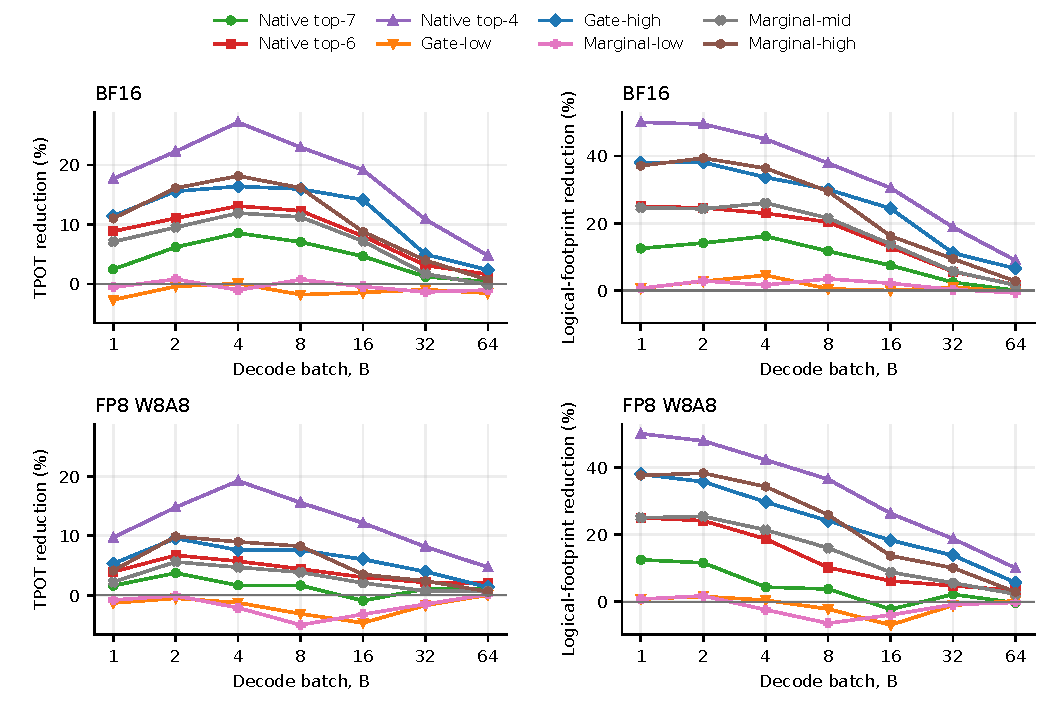
\includegraphics[width=\textwidth]{F2_formats.pdf}
\caption{F2: complete OLMoE graph matrices, 63 cells per format. Reductions use native at the same format and $B$. Every request has 128 prefix tokens and 2048 fixed outputs; TPOT excludes the first token. Logical-footprint ratios compare policies' realized trajectories via separate output-identical counted replays. They are neither DRAM savings nor same-route deletion fractions. One execution per arm supplies no independent-run uncertainty.}\label{fig:performance-r07}
\end{figure*}

Figure~\ref{fig:performance-r07} reports reductions relative to native within each format and batch. In BF16 at $B=8$, native TPOT is 8.240\,ms; marginal-mid reaches 7.312\,ms (11.26\% lower) while reducing realized logical footprint by 21.52\%. Marginal-high reaches 6.910\,ms (16.14\% lower) and reduces footprint by 29.50\%. Native top-6 is faster than marginal-mid in this run, at 7.227\,ms (12.30\% lower), despite a slightly smaller footprint reduction of 20.34\%. Thus the selected-window F3 advantage over top-6 does not establish latency dominance, and logical footprint alone does not rank execution cost.

The marginal-mid TPOT reductions across increasing $B$ are 7.09\%, 9.51\%, 11.92\%, 11.26\%, 7.18\%, 1.69\%, and $-.15$\%. Its logical-footprint reductions at $B=32,64$ are 5.72\% and 1.56\%. Marginal-high retains 3.97\% and .68\% TPOT reductions at these two batches. Gate-high is close to marginal-high at $B=8$ (15.96\% reduction) and has a larger reduction at $B=32$ (4.95\%); these small gaps have no independent-run support. Native top-4 has the largest measured TPOT reduction of the tested policies at every batch, including 22.98\%, 10.85\%, and 4.76\% at $B=8,32,64$; its stronger quality intervention cannot be ignored. Sparse gate-low and marginal-low settings have small, sometimes negative timing effects. A negative cross-policy footprint reduction can also occur because changed outputs induce different later routing, even though each local policy only removes assignments.

\begin{figure*}[tp]\centering
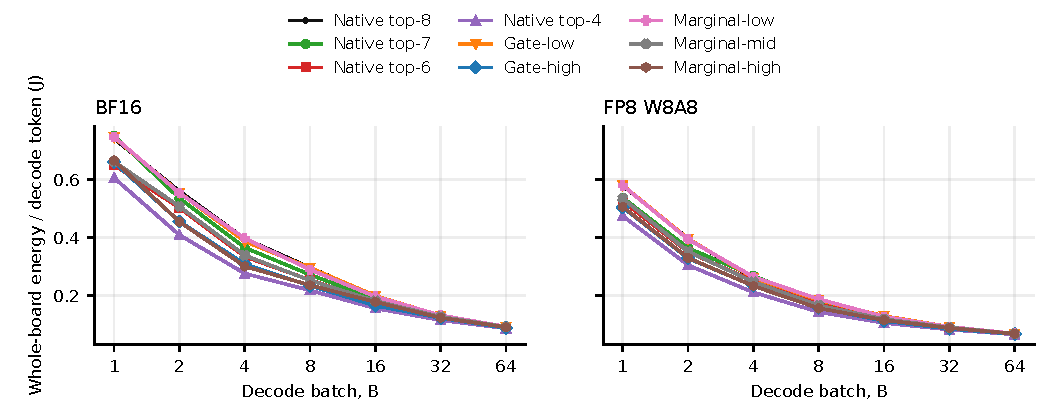
\includegraphics[width=\textwidth]{F4_formats.pdf}
\caption{F4: gross whole-board J/decode-token from separate energy replays, integrated from NVML power samples. All 63 windows per format exceed three seconds: BF16 5.61--37.14\,s and FP8 5.39--28.36\,s. Prefill and the first token are excluded; the denominator is $2047B$ decode outputs. These single-run measurements are not process-only energy, task efficiency, or quality-matched comparisons.}\label{fig:energy-r07}
\end{figure*}

Energy replays reproduce each arm's performance transcript and start sampling after all first tokens are visible, ending after the last decode output. The requested sampling interval is 50\,ms; integration uses sample timestamps and includes the host loop and NVML boundary overhead. All 126 windows exceed three seconds (BF16 5.61--37.14\,s; FP8 5.39--28.36\,s). Figure~\ref{fig:energy-r07} uses the power-sample trapezoidal integral as the primary whole-board energy measure, without attributing it to one process or converting a latency estimate into energy.

In BF16 at $B=8$, native uses .29654\,J/token and marginal-mid .25245\,J/token, a 14.87\% decrease; marginal-high uses .23602\,J/token, a 20.41\% decrease. At $B=32$, marginal-mid and marginal-high decrease J/token by 2.62\% and 5.33\%; at $B=64$ the decreases are .028\% and 1.02\%, respectively. Top-4 decreases J/token by 26.43\%, 11.72\%, and 5.61\% at $B=8,32,64$. Small changes, especially marginal-mid at $B=64$, cannot be distinguished from run-level variation with this experiment.

\paragraph{Completed FP8 performance.}
At $B=8$, native FP8 TPOT is 5.609\,ms and energy is .18182\,J/token. Marginal-mid reduces TPOT by 3.87\%, J/token by 8.24\%, and realized logical footprint by 15.99\%; marginal-high gives 8.25\%, 13.73\%, and 25.88\%, respectively. Native top-4 is faster, with 15.57\% lower TPOT and 20.80\% lower J/token, at its stronger measured quality perturbation. At $B=32$, marginal-mid/high reduce TPOT by .72/2.40\% and J/token by 2.23/4.25\%. At $B=64$, their TPOT reductions are .66/.63\%, while energy increases by .155/.006\%: effectively little observed energy change, without repeated runs to resolve small effects.

Both formats therefore show diminishing observed marginal-policy gains at larger batches, but their effect sizes differ. The same external prefix/output protocol does not fix generated content or routing across formats. Online W8A8 also changes activations and other converted linear layers, while each format has its own kernel tuning and native baseline. These measurements cannot attribute the difference solely to halving expert weight bytes, or combine short-window quality with long-trajectory performance into an equal-quality speedup.

The GPU lock did not make the host exclusive: background download activity changed across arms, so host activity and time drift remain potential confounders; no numerical correction is applied. The earlier eight-output eager diagnostic is retained as a boundary case: with untuned kernels and counters in the timed path, lower logical footprint accompanied higher TPOT. Its subsecond energy windows are not pooled with r07. Changes in tuning, graph execution, instrumentation, and workload length prevent attributing the difference between those runs to one component. Independent repeats under stable host conditions, downstream quality, and the other two models remain necessary.

\begin{figure*}[tp]\centering
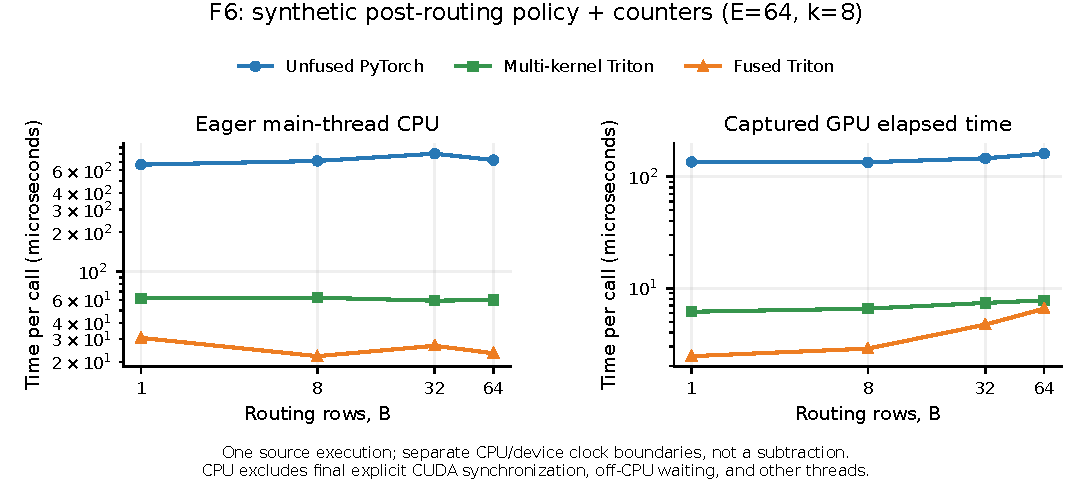
\includegraphics[width=\textwidth]{../figures/f6_r09b/F6_E_64_k_8_NVIDIA_RTX_PRO_6000_Blackwell_Server_Edition_60a476f2.pdf}
\caption{F6: measured post-routing policy and counters from r09b. Main-thread CPU consumption and captured-device elapsed time have separate clock boundaries; neither is computed by subtracting times. Both panels compare the same three implementations on synthetic routing inputs. One source execution supplies each point; inner calls are timing repetitions, not independent runs. Eager wall measurements are retained in the accompanying CSV. These are component timings, not full-model TPOT or service speedups.}\label{fig:policy-overhead-r09b}
\end{figure*}

\paragraph{Measured policy microbenchmark (F6).}
Figure~\ref{fig:policy-overhead-r09b} reports one execution on an NVIDIA RTX PRO 6000 Blackwell Server Edition with PyTorch 2.11.0+cu130. It uses fixed synthetic routing matrices with $E=64$, $k=8$, FP32 normalized selected weights, and survivor renormalization enabled. This controller-only workload has no expert weight tensors and is not a model-format comparison. The marginal policy uses tail ranks 5--8, $\tau=.15$, and $m=.20$; counters are included. At $B=1,8,32,64$, the fused Triton implementation consumes 30.785, 22.265, 26.768, and 23.432\,$\mu$s of main-thread CPU time per eager call. Captured-device times are 2.457, 2.871, 4.714, and 6.552\,$\mu$s. The unfused PyTorch implementation consumes 663.9--806.4\,$\mu$s of main-thread CPU time and 134.7--160.9\,$\mu$s of captured-device time; multi-kernel Triton consumes 59.54--62.79 and 6.15--7.78\,$\mu$s, respectively.

Each eager point averages 100 warmed calls. The \texttt{time.thread\_time\_ns} interval covers the calling thread's Python and driver submission work and ends before the final explicit CUDA synchronization. It excludes off-CPU waiting and other threads, so it is neither total process CPU consumption nor full-service CPU time. Eager wall time includes that final synchronization; the fused implementation's corresponding values are 30.923, 22.387, 26.943, and 23.623\,$\mu$s. Each device point uses CUDA events around 100 graph replays with ten policy calls per graph, excluding per-call Python dispatch and allocation. These clocks are reported independently, with no wall-minus-device estimate of CPU cost. The experiment excludes MoE GEMMs, safe dispatch alignment, attention, and full-model scheduling. The older r04 run has no thread-CPU measurement and is not backfilled. F2/F4 measure full-model behavior separately; these inner repetitions supply no independent-run confidence interval.

\subsection{Interpretation and continuing construction}
The BF16 and FP8 quality experiments support a limited observation: at some batched settings, allocating interventions to singleton tails improves the measured quality--logical-footprint tradeoff relative to a fixed-$k$ reduction. Separately, the completed graph matrices observe lower TPOT and J/token for middle/high-budget policies at several small and intermediate batches, with diminishing effects at larger batches. Stronger fixed-$k$ reduction is also faster and changes the quality tradeoff. Neither experiment shows equal-quality task acceleration: F3 has short imposed corpus continuations, whereas F2/F4 have long policy-generated fixed-length trajectories. Independent repeats under stable host conditions must test the timing and energy effects; the continuation screen and 16-problem GSM8K pilot already show changed output behavior and an observed accuracy cost, while larger held-out/task evaluations must test any quality constraint. The FP8 observations retain some batched tradeoffs but change perturbation magnitudes; they are not an independent held-out confirmation. The remaining models will test transfer.

\section{Related Work and Action-Level Comparison}
Table~\ref{tab:related} identifies the signal and action, rather than comparing method names alone. NAEE uses a calibrated ratio of the second to the first routing weight for online skipping~\cite{naee}. AdapMoE combines a layer sensitivity estimate with the routing weight and separately manages offloaded experts~\cite{adapmoe}. Both inform inference-time baselines; static expert pruning is a different intervention.

Ada-K trains an allocator to choose each token's expert count~\cite{adak}. MoE++ trains routing over ordinary and zero-computation experts~\cite{moepp}. DynMoE learns top-any thresholds and changes expert inventory during training~\cite{dynmoe}. These methods alter learning or architecture and cannot be represented faithfully by a threshold-only postprocessor. Expert Choice already makes a batch-coupled assignment by letting experts choose capacity-limited token sets~\cite{expertchoice}; it must not be called batch-independent.

SERE is the closest identified serving comparison: its primary-expert union and similarity-conditioned substitutions reduce batch-level expert redundancy~\cite{sere}. Our rule directly drops singleton tails and retains the other native assignments. It requires no functional-similarity matrix, but cannot consolidate shared secondary experts as SERE can. Whether that lower decision complexity compensates for the narrower action space remains unmeasured. The present review establishes these scoped differences, not a claim of priority or superiority.



\section{Conclusion}
Singleton occupancy separates assignment sparsity from the elimination of a batch's expert weight footprint. We implement that distinction as a budgeted tail-skipping rule and measure its behavior in OLMoE. Seven-batch occupancy measurements and teacher-forced windows in BF16 and FP8, together with BF16 rank/gate interventions, show how available actions and quality--footprint tradeoffs change with batch size. Some $B=8$ and $B=32$ validation points improve on native fixed-$k$ reduction within each format; $B=1$ does not show a uniform advantage. Perturbation magnitudes differ across formats, whose native baselines remain separate. Complete 63-cell graph matrices in each format observe marginal-mid TPOT/J-per-token reductions of 11.26/14.87\% in BF16 and 3.87/8.24\% in FP8 at $B=8$, with little energy effect at $B=64$. Stronger fixed-$k$ reduction remains faster. Different generated trajectories and multiple FP8 operator changes prevent attributing the format difference solely to expert weight bytes. The 200-window natural-completion screen is mostly length-capped, and the 16-problem GSM8K pilot has four correct answers for marginal-mid/high versus six for native. These single-run performance results and distinct quality populations do not establish equal-quality task gains. Independent performance repeats, larger held-out/task evaluations, and the remaining two target models are the next required evidence.

{\interlinepenalty=10000
\bibliographystyle{plainurl}
\bibliography{refs}}
\end{document}
